\subsection{In-place text-to-text transformation}
\label{subsec:compilation}
To remind, the previously generated extended code contains our template-based and syntactic additional programming constructs and user fine-grained code. 
This extended code itself is not compilable, executable, and debug-able. 
That is why an in-place text-to-text (T2T) transformation is needed. %XSeparation generates object-oriented code containing additional constructs for bidirectional traceability. Hence, a compilation process is needed to transform the XSeparation-generated code into machine code.
%The transformation transforms the extended code into the executable \tb{Standard code}. %to transform the XSeparation-generated code into machine code.
%The extended code shows the architecture as well as the code for fine-grained behavior.

For each component class containing our additional constructs such as ports, bindings, and state machine elements in the extended code, the T2T transformation creates an additional source code file/class, namely \ti{delegatee}, complementing with the generated extended code.
The created delegatee classes/files are in the same repository with the extended code but hidden from developer perspectives and not intended to be modified by the developers.
These delegatee files play as role of "dynamic library code files" executing the runtime semantics and logic specified by the additional constructs.

Fig. \ref{fig:delegation} shows the relationships and control flows between a component in the extended code and its corresponding generated delegatee code as followings:

\begin{itemize}[\footnotesize]
	\item A component class in the extended code owns a composite attribute typed by its delegatee class similarly to the delegation design pattern \cite{gamma1995design}.
	
	\item The execution of the component is passed off to the delegatee class through the owned composite attribute.
	
	\item The user code (e.g., state entry/exit actions or transition effects) in the component is invoked by the delegatee execution. 
\end{itemize}


 
%By this way, the final code (the code after the transformation) is composed two parts: \ti{visible files}, which are \ti{extended code files} as in Fig. \ref{fig:mappingoverview}, modifiable by programmers, and \ti{controller files}, which are automatically generated or modified by the transformation.
%The code after the transformation is then compilable, executable, and debug-able.  
%In the transformation, the extended code should be kept intact because the programmers are unlikely to see the extended code much changed after the transformation. 
%At the same time, the latter is able to map back to the model.  

\begin{figure}
	\centering
	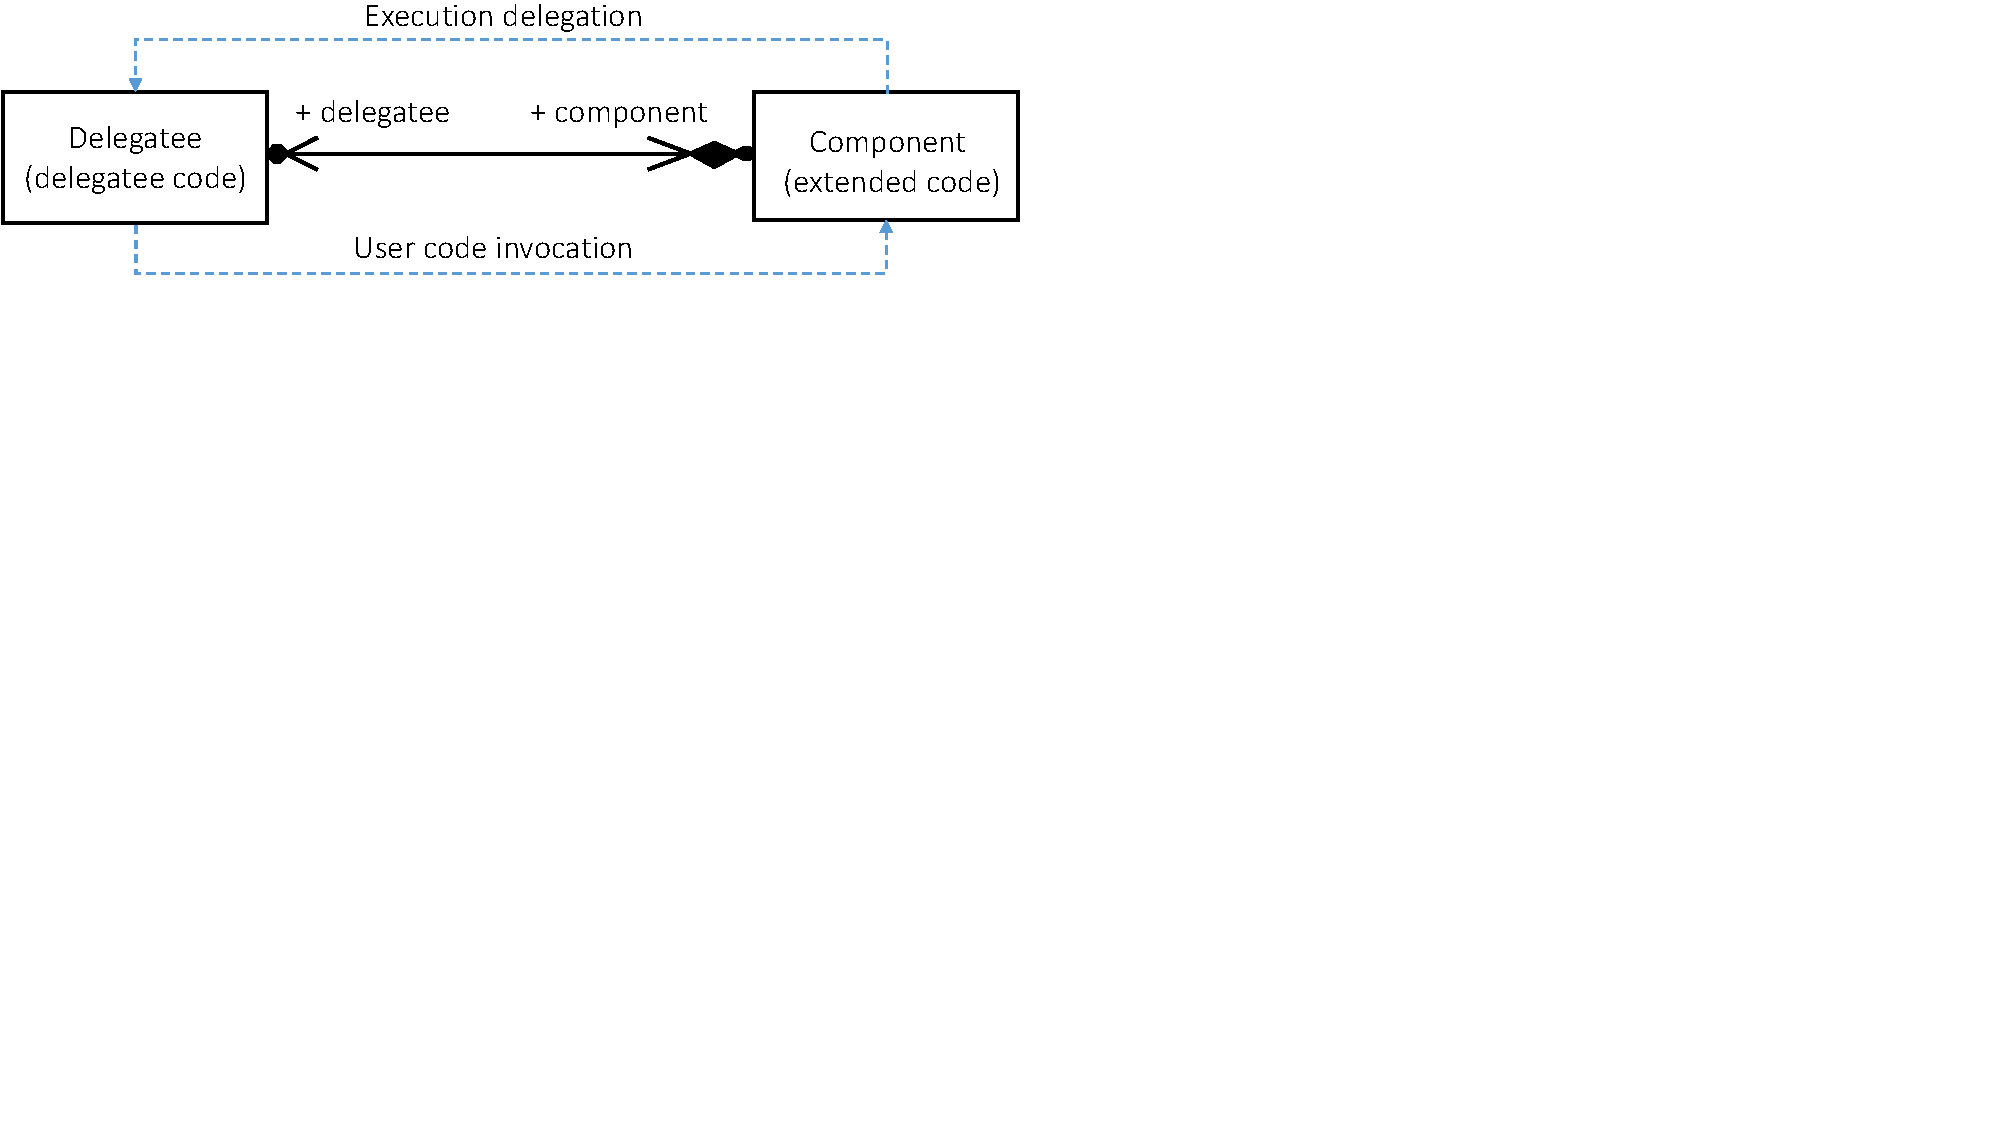
\includegraphics[clip, trim=0cm 14.2cm 16.2cm 0cm, width=\columnwidth]{figures/delegationcomponent.pdf}
	\caption{Delegation from a component to its delegatee} 
	\label{fig:delegation}
\end{figure}


%In the followings, we will explain how the controller code is generated by the transformation.

%\vspace{0.1cm}
%\noindent
%\tb{State machine controller code:}
The process of generating delegatee code from the additional constructs is actually a code generation from component-based design and state machines.
This code generation is supported by several tools such as IBM Rhapsody \cite{ibm_rhapsody} and Enterprise Architect \cite{sparxsystems_enterprise_2014}.
However, the code generated from these tools is mixed with fine-grained behavior code such as state action or transition effect code, which makes the reconstruction of state machines and component-based elements from code impossible.
Our code generation, on the other hand, completely separates the delegatee code and user code in different files.

%\vskip 0.1cm
\noindent
\tb{Port transformation:}
Each port is transformed into code elements within the corresponding delegatee as followings:

\begin{itemize}[\footnotesize]
	\itemsep0em 
	\item \ti{ProvidedPort}: A getter for getting the implementation of the port's interface.
	
	\item \ti{RequiredPort}: A setter for setting the \ti{requiredIntf} required interface attribute of the port.
	
	\item \ti{BidirectionalPort}: A setter and a getter equivalently to a required port and a provided port.
	
	\item \ti{InFlowPort}: A getter for getting the implementation of the interface containing a \ti{push} method for other components to send signals.
	
	\item \ti{OutFlowPort}: A setter for setting the \ti{intf} interface attribute of the port.
	
	\item \ti{InOutFlowPort}: A getter and a setter equivalently to an in-flow port and an out-flow port. 
\end{itemize}

Listing \ref{lst:delegatee} shows code segments for the delegatee classes associated with the producer and \ti{FIFO}.
A \ti{set\_pPush} method (lines 4-6) and two getter methods (\ti{get\_pPush} and \ti{get\_pPull} at lines 11-12) are generated for the required port of the producer and the two provided ports of the FIFO, respectively.

It is worth noting that the bodies of \ti{get\_pPush} and \ti{get\_pPull} are different because of the \ti{DataPushEvent} call event associated with the \ti{push} method (see State machine transformation for more details).


%\vskip 0.1cm
\noindent
\tb{Binding transformation:}
For each component with a configuration, a \ti{createConnections} method is created within the associated delegatee class.
Each binding in the configuration is transformed into a statement in \ti{createConnections()}.
The statement binds the interface attribute of a required port to a concrete implementation of the interface provided by the component at the other end of the connector.
Listing \ref{lst:delegatee} shows \ti{createConnections} at lines 27-32 generated for the configuration of \ti{System}.
The binding between the \ti{pPush} producer required port and the \ti{pPush} fifo provided port is transformed into a statement calling the corresponding getter and setter to assign the interface attribute of the required port to the corresponding implementation. 






%\vskip 0.1cm
\noindent
\tb{State machine transformation:} 
The transformation creates code within the delegatee class for executing the runtime logics of the state machine in the extended code.
The details of the pattern used in this transformation is presented in our previous work \cite{fullusm}.
Our transformation supports all UML State Machine concepts including transitions, states, pseudo states, and events.
This paper does not repeat this transformation but describes an example how the delegation of the state machine execution from the extended code to the delegatee works.


\begin{minipage}{0.95\columnwidth}
	\lstinputlisting[language=C++, caption={Delegatee classes of the producer and FIFO}, label=lst:delegatee,frame=f]{code/delegatees.cpp}
\end{minipage}

In Listing \ref{lst:delegatee}, the code at lines 13-22 shows how a \ti{DataPushEvent} call event is emitted and processed.
In the FIFO state machine in Fig. \ref{fig:approachexample}, an instance of the \ti{DataPushEvent} call event, which is associated with the \ti{push} method of \ti{FIFO}, is emitted if \ti{push} is called.
Therefore, whenever there is a call to \ti{push} through the \ti{pPush} port of the producer, the call event should be emitted and processed.
Hence, in the getter of \ti{FIFODelegatee} for the \ti{pPush} provided port of \ti{FIFO}, instead of returning the fifo as \ti{get\_pPull}, \ti{get\_pPush} returns the delegatee as \ti{this}.
The call to \ti{push} from the producer is then delegated to \ti{push} of \ti{FIFODelegatee} instead of that of \ti{FIFO}.
An event is then emitted and processes synchronously by the \ti{processDataPushEvent} method.
The latter checks whether the current active state is \ti{Idle} (line 14).
If so, the \ti{signalCheck} transition effect in the extended code component (lines 55-57 in Fig. \ref{fig:approachexample}) is called and followed by changing the current active sub-state to \ti{SignalChecking} (line 16).   


%To reconstruct a state machine from our generated code, we utilize the bidirectional mapping to analyze the extended code.

%Listing \ref{lst:executabletransformation} shows a code segment generated for processing the \ti{DataPushEvent} call event triggering the transition from \ti{Idle} to \ti{SignalChecking}.

 

%In the transformation, we generate a \ti{controller} class for each class containing bindings or state machine elements and create connections between parts through ports (see lines 15-19 and 5-10 in Listing \ref{lst:executabletransformation}).
%The fine-grained code in the extended code will be called by the controlling (standard) code or the controller classes.
%Listing \ref{lst:executabletransformation} shows the generated standard code.
%\ti{SystemController} is associated with \ti{System} by referring to the system object through a pointer \ti{pSys}. 
%This class also declares a \ti{controller} attribute typed by \ti{FIFOController} associated with \ti{FIFO}.
%During code execution, the required and provided interface of the \ti{pPush} ports of \ti{Producer} and \ti{FIFO}, respectively, refer to the controller of \ti{FIFO}.
%The \ti{required} and \ti{provided} attributes are actually declared within the port constructs as described in \ref{subsec:bimapping}.
%If a programmer wants to call the \ti{push} method provided by \ti{FIFO}, she/he only needs to write \ti{pPush.required->push(data)}, which will call the \ti{push} method implemented by the FIFO controller.
%The \ti{pPush} ports refer to \ti{controller} because a call event associated with \ti{push} is declared within \ti{FIFOStateMachine}. 
%In order to process the event emitted by calling the \ti{push} method of \ti{FIFO} through its \ti{pPush} port, an appropriate method for event processing is called before the call to \ti{push} of \ti{FIFO} through a reference to \ti{FIFO} (lines 20-23).



%The interfaces of the \ti{pPull} ports refer to the fifo (lines 8-9) because no event should be emitted and processed in case of an invocation to the \ti{pull} method.  
%Fig. \ref{fig:compilerarchitecture} shows the transformation process consisting of \tb{Structure code transformation} (SCT) and \tb{Behavior code transformation} (BCT). 

By this transformation, on one hand, the programmers can execute and debug the extended code and modify the architecture at the code level while keeping the mapping between the model and the code bidirectional.
On the other hand, the model can be reconstructed from the extended code by utilizing the proposed bidirectional mapping if there are modifications in the extended code, either to the architecture or the fine-grained behavior.

In the next section, we will show how the modifications in the model and the extended code can be synchronized by our synchronization mechanism.




%\begin{figure}
%	\centering
%	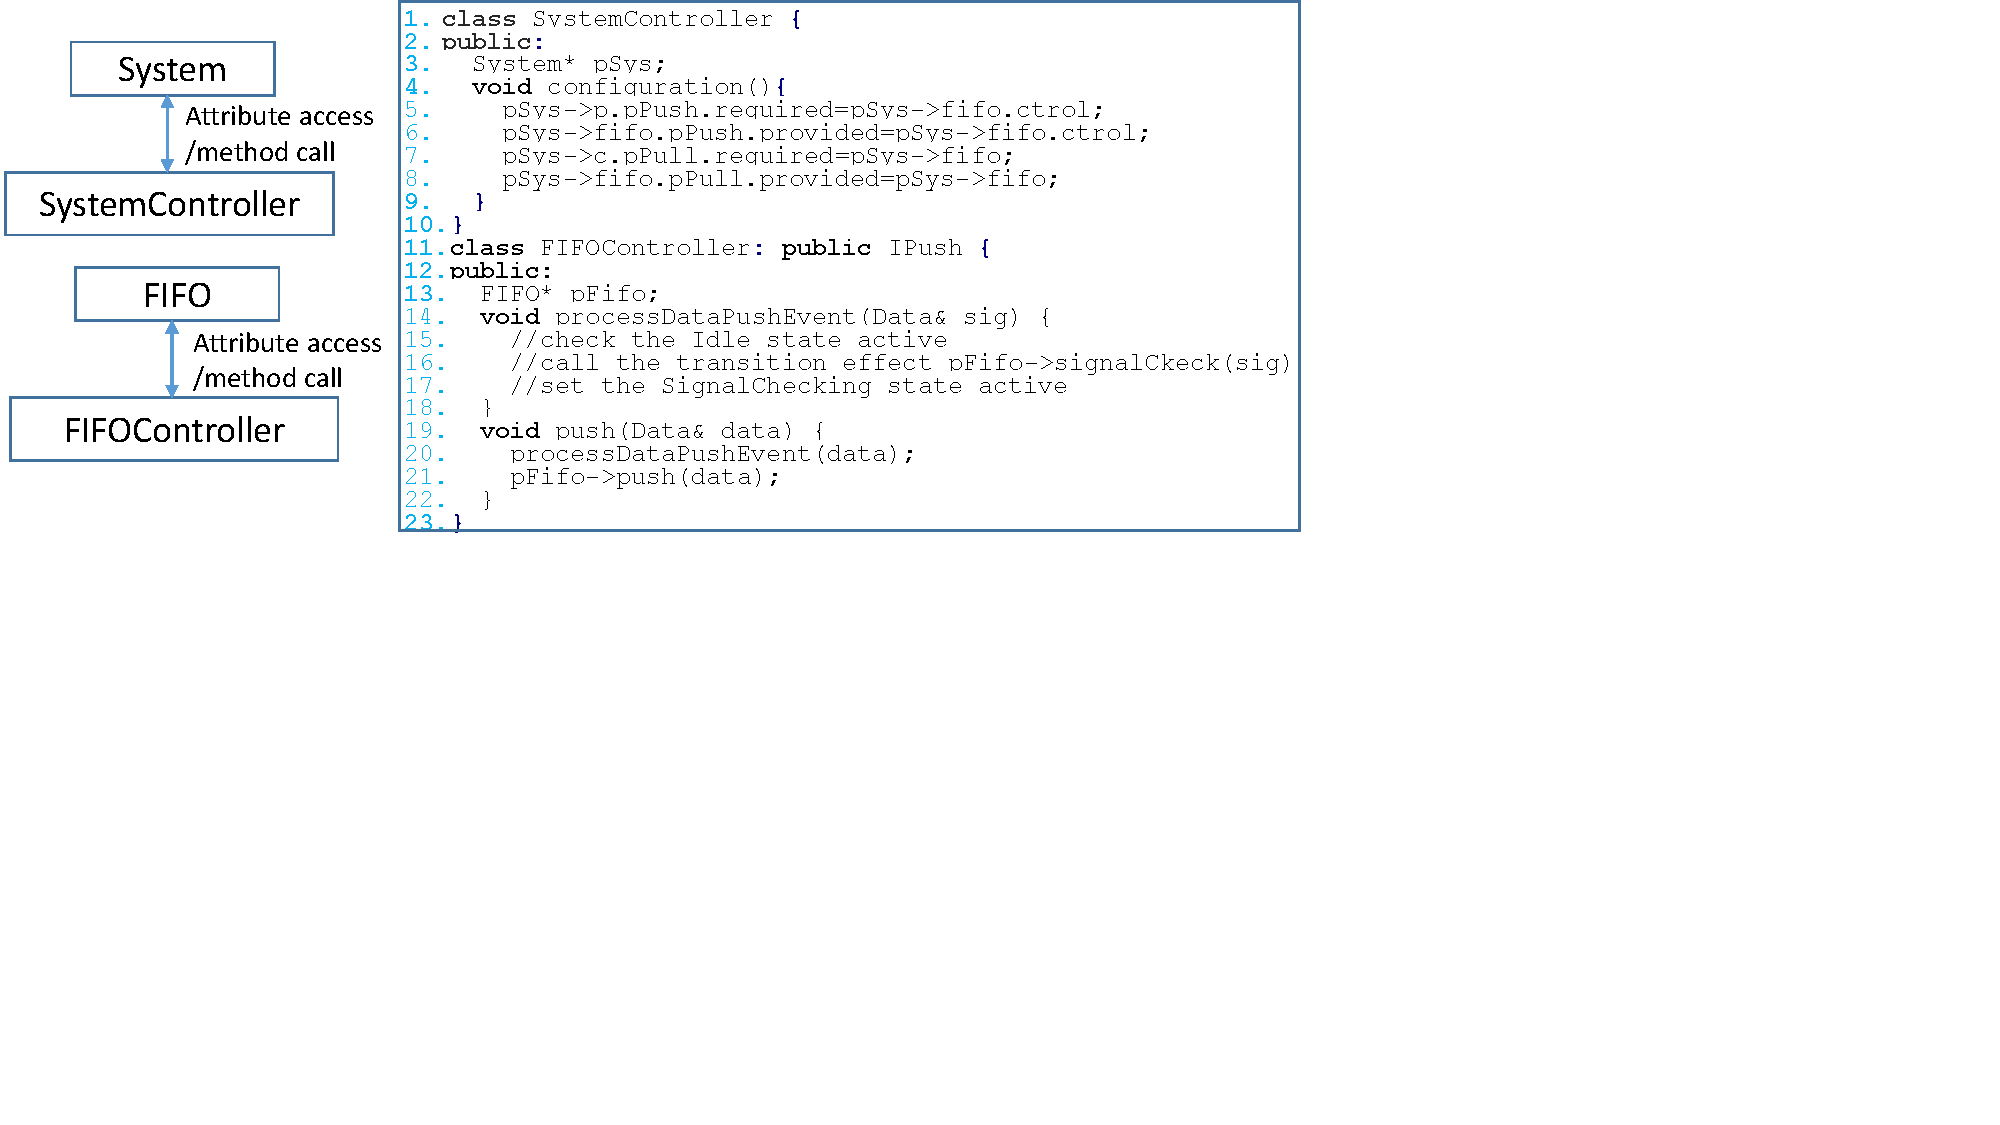
\includegraphics[clip, trim=0cm 10.1cm 11.2cm 0cm, width=\columnwidth]{figures/executabletransformation.pdf}
%	\caption{XSeparation compiler's architecture} 
%	\label{fig:compilerarchitecture}
%\end{figure}


%\vskip 0.1cm
%\noindent
%\tb{Structure code transformation:}
%A verification is firstly executed to check the well-formedness of components and ports.
%We basically verify three port rules: (1) every port with a required interface or provided data must be bound to another port; (2) if two ports are connected by a assemble connector, the provided interface/data of one port must identical to or an extension of the required interface/data of the other port; and (3) if the connector is delegate, the provided interface/data of one port must identical to or an extension of the provided interface/port of the other port; 
%Once the rules are verified, executable code can be generated. 
%SCT transforms the additional structural constructs into standard code.
%Fig. \ref{fig:compilerarchitecture} shows a segment of standard code generated from the producer-consumer example.
%Each port with required interface is transformed into a pointer attribute (lines 12 and 15) while each part into an object attribute (lines 3-5).
%A configuration method is transformed into a method \ttt{configuration}.
%A binding (bindPorts) in the configuration is transformed into an assignment which refers the pointer associated with a port with provided interface to the corresponding implementation.
%For example, the \ti{pPush} pointer of \ti{Producer} is referred to the fifo, which implements the \ti{IPush} interface (line 7). 
%When a method is called through a port, for example \ttt{push} through the \ttt{pPush} port, the corresponding method implemented in FIFO is invoked. 


%\vskip 0.1cm
%\noindent
%\tb{Behavior code transformation:}
%It transforms the behavioral constructs for state machines into standard code similarly to code generation approaches from UML State Machines in MDE tools such as Rhapsody.
%Our goal is to support all of the features of state machines.
%However, the existing tools only support a subset of state machine concepts, e.g. Rhapsody does not support junctions, truly concurrent execution of orthogonal regions \cite{ibmdiff}, and all of the UML event types.
%UML events are not supported 
%The concurrency of the orthogonal regions is often implemented sequentially \cite{Badreddin2014}. 
%In addition, there are other issues such as event processing speed, executable file size, and UML semantic-conformance defined by a recent work on the Precise Semantics of State Machine (PSSM) \cite{OMG2015}.
%XSeparation compiler supports full features of state machines.
%XSeparation compiler has following features.

%\begin{itemize}[\footnotesize]
%We extend an existing code generation pattern with the use of IF/ELSE to support all of the state machine features. 	
%We currently evaluate the semantic-conformance of  A recent specification formalizing the precise semantics of UML State Machine is under standardization of OMG.
%It defines a test suite with 66 test cases for certifying the conformance of runtime execution of code generated from UML State Machines.
%We have experimented XSeparation compiler with the test suite.
%The traced execution results of 62/66 test cases comply with the standard and are a good hint that the execution is semantically correct.
%Due to space limitation, the details of pattern and evaluation for state machine runtime execution semantics are not presented in this paper.

%\vskip 0.1cm
%\noindent	
%\tb{State machine configuration:} XSeparation allows to configure the event queue size and periodic time for evaluation of change events.

%\vskip 0.1cm
%\noindent	
%\tb{Event API:} Generated code in XSeparation compiler provides APIs for environment code to invoke operations or send data signals through component ports.
%	The invocations and sending will automatically fire events for state machines to process.
%\end{itemize}

%\vskip 0.1cm
%\tb{Runtime}
%Asynchronous events are stored in an event queue managed by the component at runtime.
%Furthermore, the boolean expression of ChangeEvent is periodically evaluated.
%The size of the queue and the periodic evaluation time can be configured within the topology of the state machines.
%Others such as event priorities are configurable but not implemented for the moment.
%Lines 32-35 in Listing \ref{lst:fifostatemachine} configures the size of the queue as 50 and the periodic evaluation time is 20 millisecond.
%Note that this configuration is different from the structure configuration, which is used for wiring different components through explicitly defined ports.
%UML, however, remains abstractly and does not specify these configuration values.
%We then define a profile support for UML State machine configuration.
%Fig. \ref{fig:fifostatemachine} shows the configuration values annotating the state machine example.

%In the next section, XSeparation will be implemented as an extension of the Papyrus modeling tool and evaluated by developing a case study of software application for LEGO.